
\title{Physics 2D report}
\author{
Keith Goh Guan Da(1003334)\\
Cheow Pak Leng Josiah (1003602)\\
Yang Peng (1003776)\\
Jessica Davinia Layardi (1003675)\\
Xu Shuangyi (1002952)\\
}
\date{\today}

\documentclass[10pt]{article}
\usepackage{graphicx}
\usepackage{appendix}

\graphicspath{ {./images/} }

\begin{document}
\maketitle
\newpage
\begin{abstract}
In this project, our group hopes to create a temperature predicting sensor using our knowledge from engineering in the physical world and digital world. The temperature sensor should be able to predict temperatures between 10 to 60 degrees celcius within a temperature range of 1 degree in less than 10 seconds.
\end{abstract}
\section{Introduction}
\paragraph{Problem}\mbox{} \\
Conventional thermometer requires extensive amount of time to be at thermal equilibrium with the object to accurately measure its temperature.
Aim: To write a program that reads data from a given temperature sensor and uses machine learning and statistical analysis to predict the actual temperature of a water bath accurately within a reasonable time frame.
\paragraph{Assumptions}\mbox{} \\
The value of $\tau$ is given by
\begin{equation}
\tau=\frac{\mathrm{C}_{\mathrm{s}}}{\lambda}
\end{equation}
However since the heat capacity of water is between 4150$\frac{J}{KgK}$ and 3980$\frac{J}{KgK}$ for water and we are using the same setup hence having the thermal conductance $\lambda$ for each experiment. We assume that tau is a constant for such a small range of temperatures.
We assumed temperature throughout the experiment is constant by neglecting any heat transfer via convection and conduction between the water, container and surroundings.
This is through the use of a thermal flask which minimizes the heat tranfer to the surrounding.
We also assumed that temperature gradient is 0 which means temperature is  the same throughout the water after stirring it.

\paragraph{Methodology}
\begin{enumerate}
\item Data collection:\\
In order to collect the necessary data to see whether the value of  $\tau$ changes when temperature varies, we carry out the following steps:
\begin{enumerate}
\item Fill thermal flask with water and place the thermometer into the water
\item Adjust the temperature using hot and cold water. To get a consistent temperature,ensured that the water is well mixed by stirring. Record the temperature with the thermometer once the temperature has reached a steady temeperature.Prepare the python program for temperature measuring.
\item Place temperature sensor into water and concurrently start the temperature measuring program.
\item Let the temperature measuring program run, it will record down the time elapsed, and corresponding temperature,  in the corresponding csv file.
\item Repeat steps 2-5 with different temperatures of water to get at 20 datasets of $\ln\frac{\mathrm{T}_{\mathrm{w}}-\mathrm{T}_{\mathrm{s}}}{\mathrm{T}_{\mathrm{w}}-\mathrm{T}_{\mathrm{amb}}}$ against time.
\end{enumerate}
\item Set up for data collection:\\
Setup in Appendix A
\item Find the value of $\tau$:\\
From the time dependent thermodynamic First Law, we derive the relationship of  Ts and Tw: (According to the pre-analysis worksheet)
\begin{equation}
\mathrm{C}_{\mathrm{s}} \frac{\mathrm{dT}_{\mathrm{s}}}{\mathrm{dt}}=-\lambda\left(\mathrm{T}_{\mathrm{s}}-\mathrm{T}_{\mathrm{w}}\right)
\end{equation}
the initial  Ts=Tamb , thus solving the first order differential equation above we get:
\begin{equation}
\mathrm{T}_{\mathrm{s}}=\mathrm{T}_{\mathrm{w}}-\left(\mathrm{T}_{\mathrm{w}}-\mathrm{T}_{\mathrm{amb}}\right) \mathrm{e}^{-\frac{\mathrm{t}}{\tau}} \int_{0}^{\mathrm{t}} \frac{1}{\mathrm{C}_{\mathrm{s}}} \mathrm{dt}
\end{equation}
substitute $\frac{\mathrm{C}_{\mathrm{s}}}{\lambda}=\tau$ into the equation above to find the relationship between and time(t):
\begin{equation}
\tau=-\frac{t}{\ln \frac{\mathrm{T}_{\mathrm{W}}-\mathrm{T}_{\mathrm{S}}}{\mathrm{T}_{\mathrm{W}}-\mathrm{T}_{\mathrm{amb}}}}
\end{equation}
since the value of $\tau$ should be a constant, we tried to find the value of tau by processing the $\ln\frac{\mathrm{T}_{\mathrm{w}}-\mathrm{T}_{\mathrm{s}}}{\mathrm{T}_{\mathrm{w}}-\mathrm{T}_{\mathrm{amb}}}$ against time for many sets of data using linear regresion.
\end{enumerate}
\section{Minimizing experiment errors}
Since we assumed Tw is constant throughout each experiment, we need to minimize the heat loss by using a good thermal flask.\\
Repeat the experiment 23 times using water of different temperatures and record  Ts for up to 30 seconds. Calculate the average value of all the $\tau$ obtained from each single experiment to reduce errors caused by human. Based on the equations we obtained above, plot Ts  vs time and $\ln \frac{\mathrm{T}_{\mathrm{w}}-\mathrm{T}_{\mathrm{s}}}{\mathrm{T}_{\mathrm{w}}-\mathrm{T}_{\mathrm{amb}}}$  vs time graphs in which we can use the absolute value of the slope to 	obtain $\tau$.
\section{Result and Discussion}
Referring to graphs in Appendix C,
 We can see from the plot that after 50s,the values taper off  which means that there is no heat transfer between the sensor and the water after 50s. Hence using the values obtained from first 50 secs, we plot the linearized version of the graph.\\
Consider the equation $\mathrm{t}=-\tau \ln \frac{\mathrm{T}_{\mathrm{w}}-\mathrm{T}_{\mathrm{s}}}{\mathrm{T}_{\mathrm{w}}-\mathrm{T}_{\mathrm{amb}}}$. If $\tau$ is a constant, it would represent the negative gradient of the plot and the plot of $\ln \frac{\mathrm{T}_{\mathrm{w}}-\mathrm{T}_{\mathrm{s}}}{\mathrm{T}_{\mathrm{w}}-\mathrm{T}_{\mathrm{amb}}}$
should show a linear relationship.After processing the data using the code in the jupyter notebook, the data shows that an $r^2$ value of only 0.895 for the combined dataset. Hence it shows that between the values experiments the $\tau$ value actually changes quite a bit. We used this value of $\tau$ which is 18.9 to estimate the value of the temperature of the water. However our results were not optimal. This is done using the formula.
\begin{equation}
  \tau\frac{dT_s}{dt}+T_s(t)=T_w
\end{equation}
The results of which are shown in Appendix E.
\section{Evaluation}
There could be some factors which may disprove our conclusion, although experimental data shows a high probability of $\tau$ being a constant under different temperatures. This because when the value of tau is individualised for the indiviudal temperatures.We are actually able to get a $r^2$ value of 0.99 for most experiments. Hence for individual experiments the relationship is very linear. Hence we know that $\tau$ has a strong linear relationship.
\section{Conclusion}
From our results we can draw a few conclusions that may lead to the error our of experiments.
{\begin{enumerate}
  \item There is a problem with our assumption which heat capacity is a constant and that heat capacity is actually a significant factor in the value of $\tau$.
  \item Human error is quite a significant error through our data colleciton. The probe was put in not at the start time of the experiment.However this was minimized but taking the timing of the start of experiment as the first temperature before the rise/fall of temperature.
  \item The temperature sensor is not accurate enough hence,the intervals between the collection of data was too large and hence contributed to an inaccurate collection of results
  \item There is significant heat transfer with the surroundings.

\end{enumerate}}
Hence we decided to calculate the temperature of water using another method. We used a linear regression of the temperature of the water between 0 to 8 seconds,obtaining an equation $c1+2t=Tw$ We then multiplied it by a fixed t which was done through experimentation and found to be around 16.5. Using our new method the results were found to have an accuracy rate within our range of +-1  95\% of the time. This is shown in Appendix E
\newpage
\begin{appendices}
\huge
Appendix
\normalsize
\section{Setup}
\begin{figure}[h]
\caption{picture of setup of experiment}
\centering
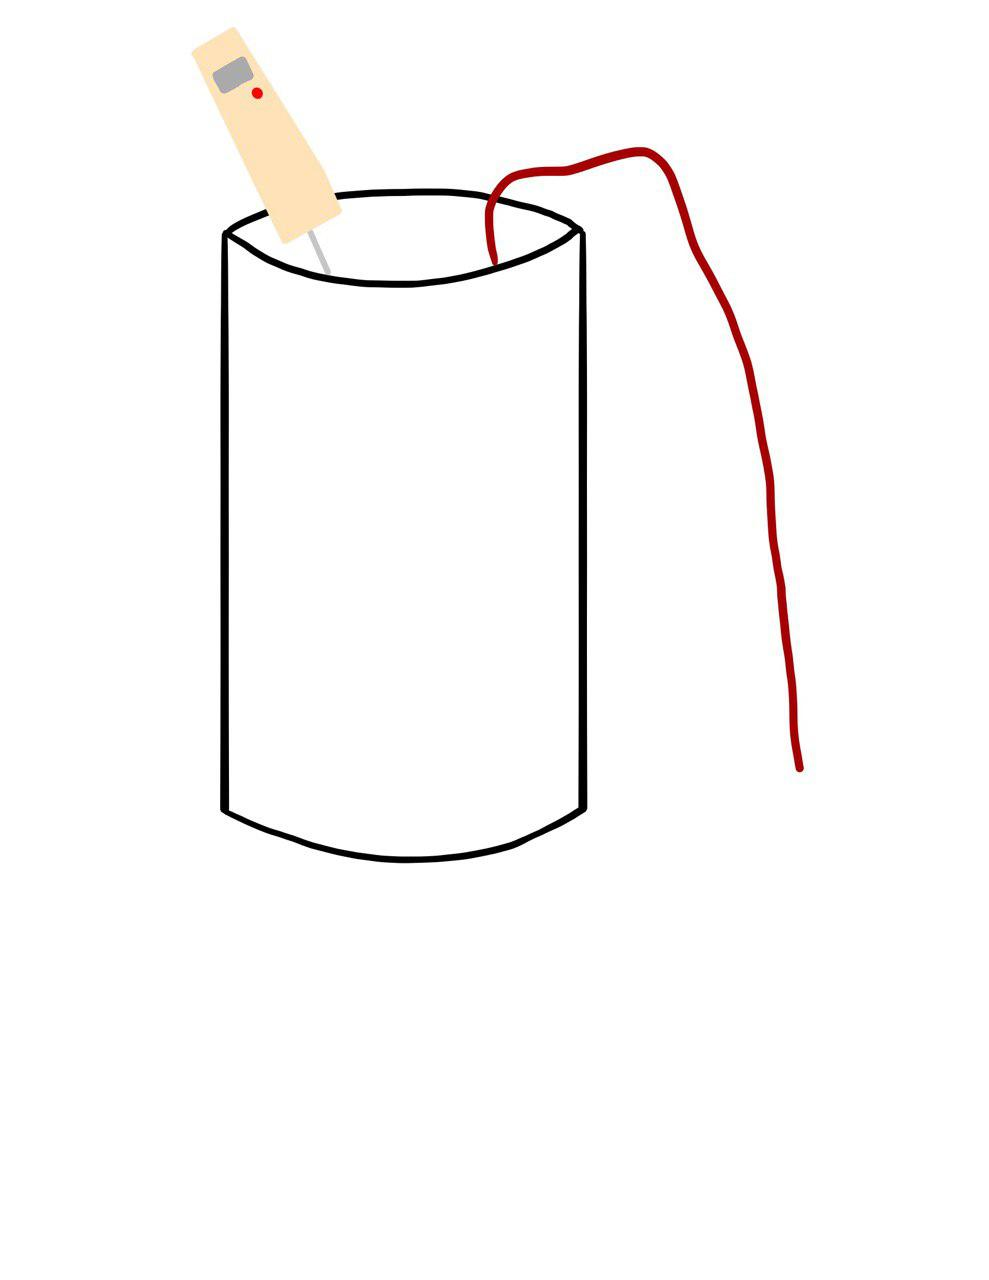
\includegraphics[scale=0.3]{3}
\end{figure}
\newpage
\section{Worksheet}
This is a scanned copy of our worksheet
\begin{figure}[bp!]
\caption{picture of front of worksheet}
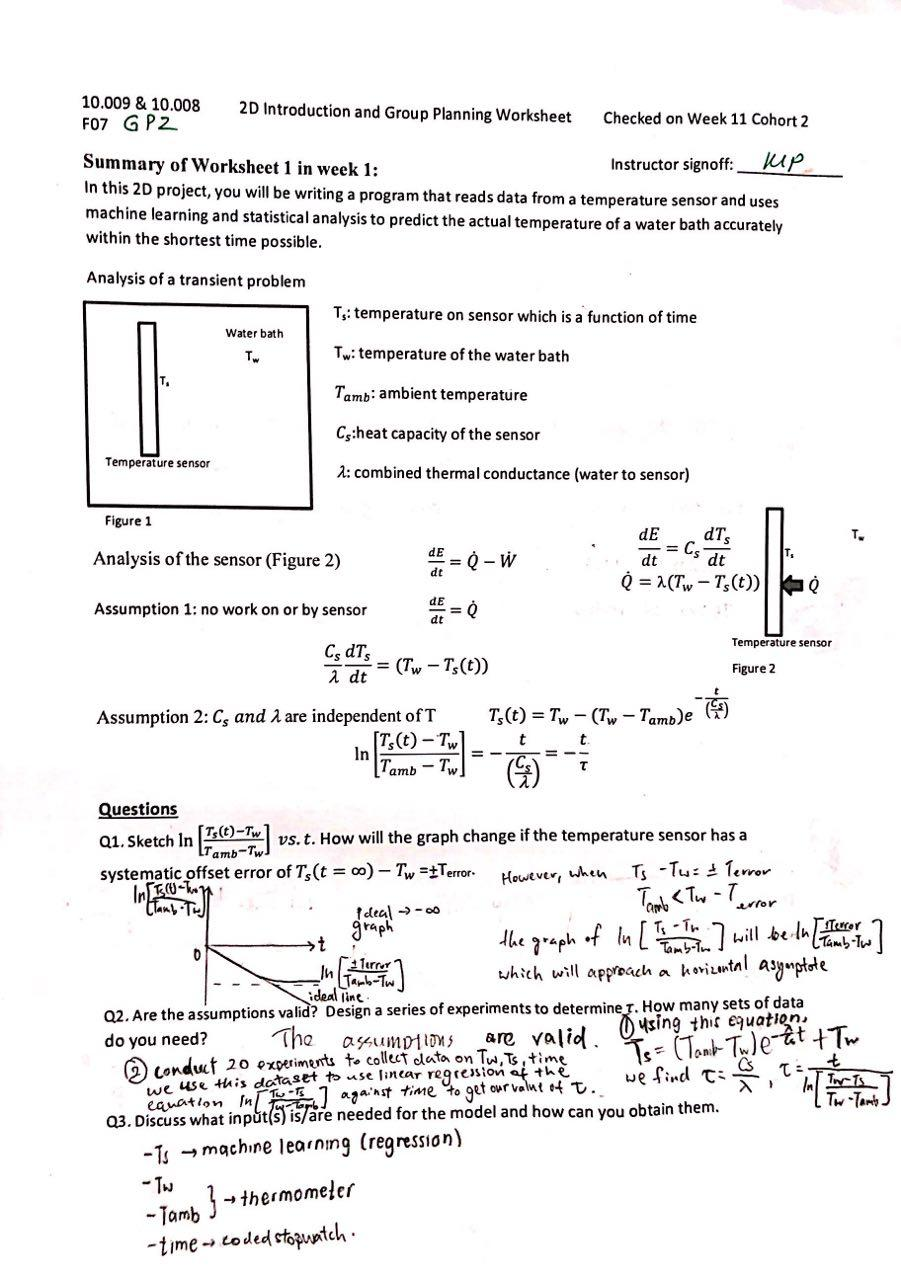
\includegraphics[scale=0.9]{9}
\end{figure}
\begin{figure}[bp!]
\caption{picture of back of worksheet}
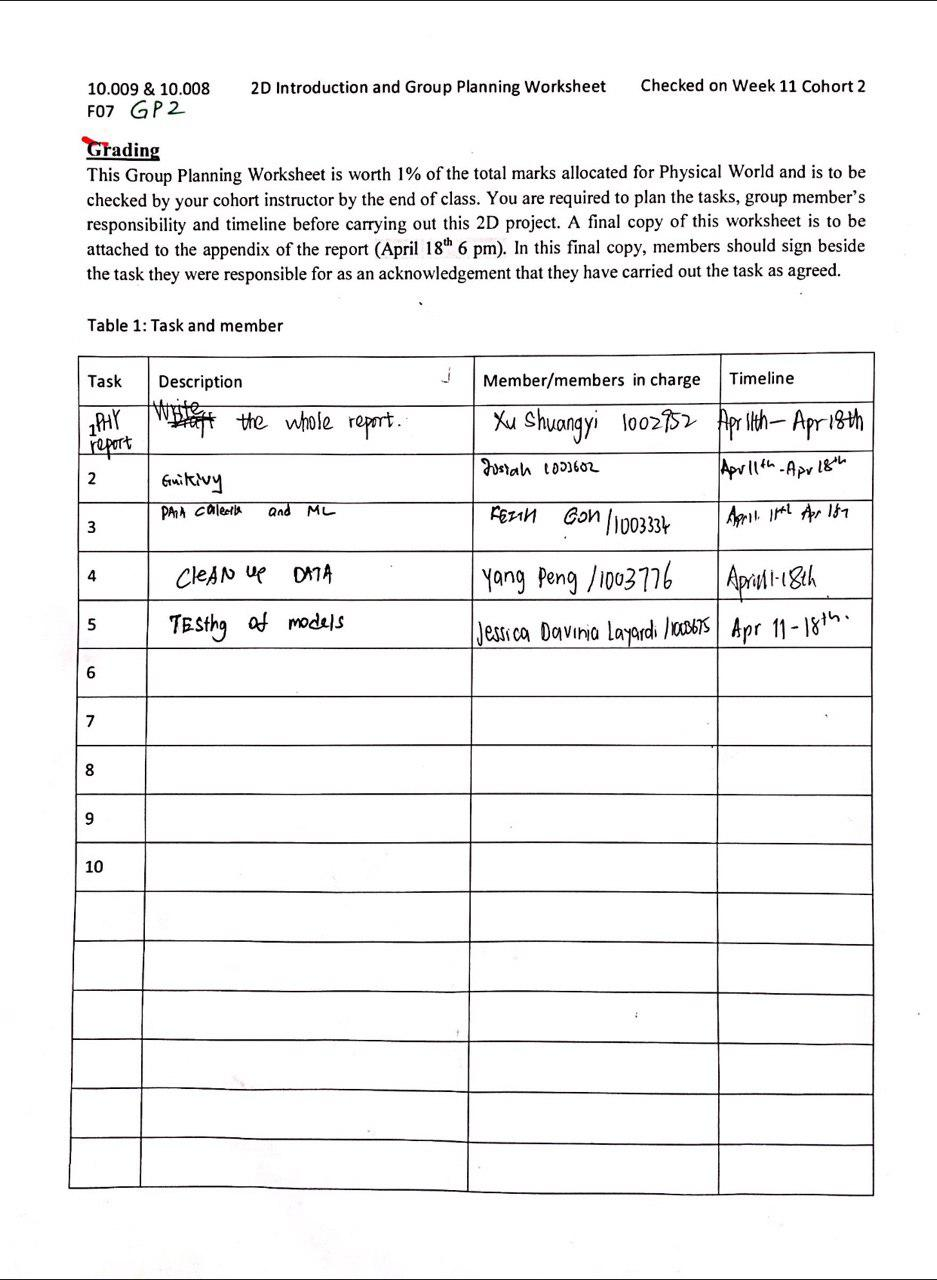
\includegraphics[scale=0.35]{2}
\end{figure}
\newpage
\section{Graphs of experiment 8}
This are the processed graphs for our experiment 8
\begin{figure}[h]
\caption{graph of experiment 8 against time}
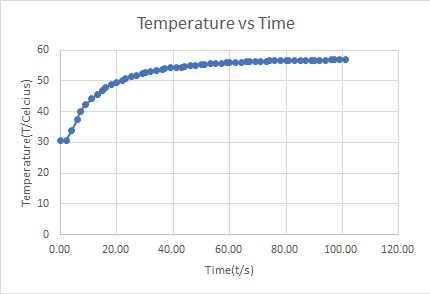
\includegraphics{4}
\caption{graph of experiment 8 linearized against time}
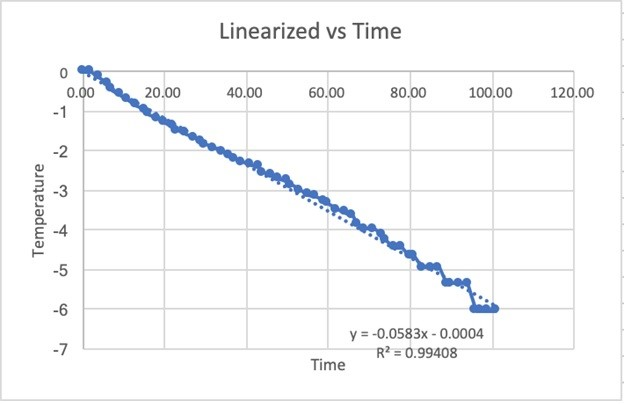
\includegraphics{5}
\end{figure}
\newpage
\section{plots of all expriments}
\begin{figure}[h]
\caption{graph of all experiments against time}
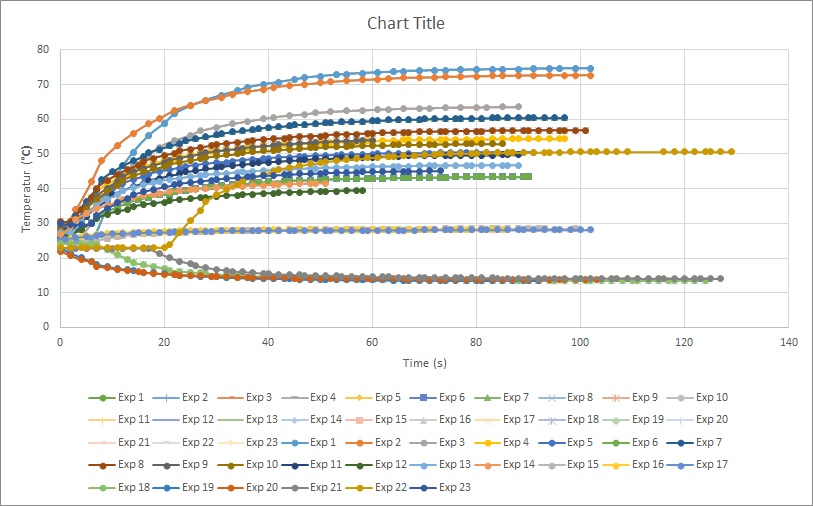
\includegraphics[scale=0.5]{6}
\end{figure}
\newpage
\section{results}
\begin{figure}[h]
\caption{results f}
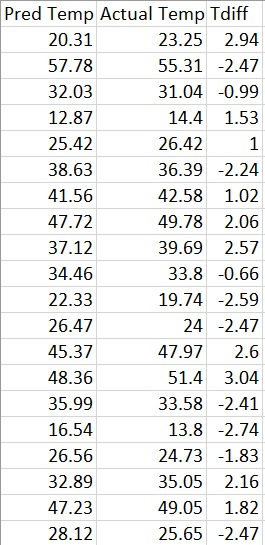
\includegraphics[scale=0.8]{7}
\caption{results of first algorithm to predict temperature}
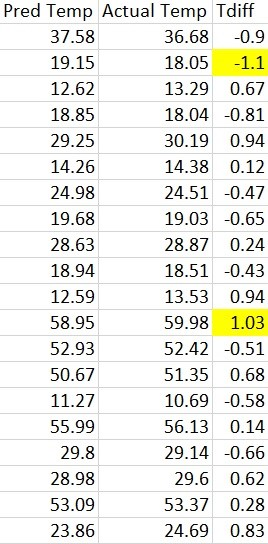
\includegraphics[scale=0.8]{8}
\caption{results of second algorithm to predict temperature}
\end{figure}
\end{appendices}
\bibliographystyle{abbrv}
\bibliography{main}
\end{document}
